\section{Testing}
    Testing is an integral part of any non-trivial piece of software today. It offers an insight into previously unknown or unnoticed problems, and is a significant portion of the quality assurance process surrounding many current software products. Although it cannot eliminate all possible issues, considering that the test case permutations are virtually endless, careful choices of input data and scenarios can cover large portion of possible code paths.
    
    \textsc{Liebert}, being rather large and complex, contains a potent set of various tests to ensure additional safety than what \textit{Rust} can offer. Testing is a first-class citizen in \textit{Rust}. It is integrated into the language and compiler, and additionally has full support in the \textit{Cargo} package manager. To execute all tests, one can simply call \textit{cargo test}, instead of the usual \textit{cargo build}. This will set-up the testing environment and run all tests in the current project, long-running ignored tests can be included by adding the \textit{--ignored} switch.
    
    
    \subsection{Unit tests}
        Unit tests are specialized tests focusing on very small and specific parts of software. Usually, a single unit test is used for testing a single function. A very unfortunate side effect of the heavy threading pattern in \textsc{Liebert} is that there aren't many functions which could be easily tested using unit tests. A great portion of functions consist of spawning a new thread executing a closure, additionally they require complex parameters such as the configuration structure (\autoref{sec:config}). As many of these closures aren't very long, most functionality is present directly within the closure, without calls to other functions. Consequence is that these functions often represent an entire module instead of a simple task, and are therefore more suitable for integration testing (read more in next section). This is an explicit fault of \textsc{Liebert}, and refactoring the code into more fine-grained functions would be beneficial, however is out of scope of this project. Additionally, due to the nature of the project, some functions cannot be tested in the traditional unit test sense where an exact result is specified. If we, for example, take the \textit{get\_current\_jiffies} function of the built-in CPU gatherer, we can see that it's output is tied to the very current state of the system, therefore an exact expected value cannot be specified.
        
        Even though the aforementioned issues are widespread in the project, unit testing is still used throughout. These tests can be created effortlessly in \textit{Rust}. In fact, compared to most other languages, they don't even require a separate file. Unit tests can be written within each file where testing is required, keeping all related code in one place.
        
        \begin{figure}[!htb]
            \centering
            \begin{BVerbatim}
#[test]
fn t_rrd_from_str() {
    assert_eq!(Some(0), rrd_from_str("0"));
    assert_eq!(Some(1), rrd_from_str("1"));
    assert_eq!(Some(99999999999), rrd_from_str("99999999999"));
    assert_eq!(None, rrd_from_str("U"));
}
            \end{BVerbatim}
            \caption{A simple unit test in the \textit{util} module}
            \label{fig:unit-test}
        \end{figure}
        
        To illustrate, we can take a look at the very simple unit test shown in \autoref{fig:unit-test}. This test is for the function \textit{rrd\_from\_str} int the \textit{util} module. Its purpose is to receive a string, and output a more suitable binary representation of the contents (an \textit{Option$<$i64$>$}). Most notable part of this code is the \textit{\#[test])} macro. This tells the compiler that the function is part of the test suite, and should be run accordingly. Moreover, the block of tests is prefaced with a \textit{\#[cfg(test)]} macro which prevents it from getting compiled into the release binary, and is only present within the testing environment.
    
    
    \subsection{Integration tests}
        Integration testing is usually one of the middle steps in the testing chain. It uses modules which previously underwent unit tests, and submits the module as a whole to more comprehensive tests. \textit{Rust}, once again, ships with integration testing in mind. Aside from including tests directly within each module, it allows the creation of a specialized \textit{tests} folder, which can be used for other purposes (such as integration tests). \textsc{Liebert} utilizes this types of tests as well. Once more, we can look at the built-in CPU gatherer module and its integration test. Due to the length and complexity it is not included in here, but you can find it in \textbf{Appendix F} (\autoref{apd:integration-test}). This test resides in the \textit{tests/builtin\_cpu.rs} file, and is run along with other tests during \textit{cargo test}. A major difference of the tests within the \textit{tests} directory is that they are all compiled as different \textit{crates} (packages) from the main application. This allows, for example, integration testing of libraries where the tests act as actual external consumers. Running \textit{cargo test} on \textsc{Liebert} results in what can be seen in \autoref{fig:test-result}.
        
        \begin{figure}[!htb]
            \centering
            \begin{BVerbatim}
Compiling liebert v0.2.0 (file:///home/.../liebert)
running 19 test
test agent::connector::tests::t_should_abort ... ok
test agent::plugins::builtin_cpu::t_get_current_jiffies ... ok
...
test result: ok. 19 passed; 0 failed; 0 ignored; 0 measured
...
running 7 test
test plugin_builtin_cpu ... ok
test plugin_builtin_memory ... ok
...
test result: ok. 7 passed; 0 failed; 0 ignored; 0 measured

 Doc-tests liebert
running 0 tests
test result: ok. 0 passed; 0 failed; 0 ignored; 0 measured
            \end{BVerbatim}
            \caption{Excerpt from the output of the \textit{cargo test} command}
            \label{fig:test-result}
        \end{figure}
        
        We can notice a curious \textit{Doc-tests} section at the end of \autoref{fig:test-result}. This are special kind of tests that are used for testing \textbf{examples in documentation}, to maintain documentation validity. Rust encourages documenting libraries through special code blocks, including examples of usage, and the compiler can automatically generate standardized documentation in HTML format based on them. This is a very unusual occurrence in a programming language, however it is a tremendous time-saver as the documentation for all libraries looks exactly the same. Note that \textsc{Liebert} does not utilize this functionality as it is not a library, and function-related documentation does not provide any meaningful information to the user.
        
        
    \subsection{Continuous integration}
        As I am a huge proponent of continuous integration and delivery, and automation in general, \textsc{Liebert} benefited from this as well. Its GitHub repository (which itself is an automated mirror of the official GitLab repository), is linked to \textbf{Travis CI}\footnote{Travis CI is a cloud CI/CD platform offering free tier for open-source projects}. Whenever any new commits are pushed to the repo, it is automatically built and tested on Travis CI against all three \textit{Rust} release channels: stable, beta, and nightly (example result in \autoref{fig:travis}). Additionally, the results of the CI run, as well as push notifications, are automatically posted to various communication channels such as \textit{Slack}.
        
        \begin{center}
            \begin{figure}[!h]
                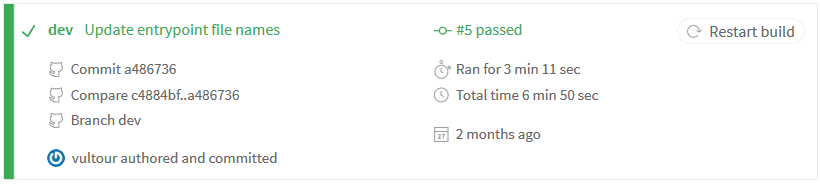
\includegraphics[width=\textwidth]{liebert-travis.png}
                \caption{An example result of a Travis CI build}
                \label{fig:travis}
            \end{figure}
        \end{center}